\documentclass[12pt]{article}

\usepackage[a4paper, left = 1.5cm, right = 1.5cm, top = 1.5cm, bottom = 1.5cm]{geometry}

\usepackage{amsmath}
\usepackage{amssymb}

\usepackage{pgfplots}
\usepackage{pgfplotstable}
\pgfplotsset{width=15cm,height=7cm,compat=newest}
\usepgfplotslibrary{fillbetween}

\usepackage{mathtools}

\usepackage{enumitem}

\usepackage{graphicx}

\usepackage{diagbox}

\usepackage{karnaugh-map}

\usepackage[T1]{fontenc}

\usepackage{listings}
\usepackage{xcolor}
\lstset{
	language = Python,
	backgroundcolor=\color{black!5}, % set backgroundcolor
}

\renewcommand{\baselinestretch}{1.5}

\renewcommand\thesection{\arabic{section}.}

\usepackage{tocloft}
\cftsetindents{section}{0em}{2em}
\cftsetindents{subsection}{0em}{2em}
\renewcommand\cfttoctitlefont{\hfill\Large\bfseries}
\renewcommand\cftaftertoctitle{\hfill\mbox{}}
\setcounter{tocdepth}{2}

\begin{document}
\begin{titlepage}
\centering
\vspace*{\fill}
\huge CS553: Cryptography\\
\LARGE Assignment 5: Solutions\\
\Large Rohit Das (11910230)\\\vspace{0.8cm}
\today
\vspace*{\fill}
\end{titlepage}

\section{DC of Sypher002}
\begin{large}
12-bit key = (4||e||6)\\
Since we need the characteristic $f \xrightarrow{\text{S}} d$, the difference for the message pairs taken is "f".\\
Below is the matrix generated for guesses of $k_2$, for which $v_{0}^{'} \, \oplus \, v_{1}^{'} = d$:

\begin{center}

\begin{tabular}{c|*{16}{p{0.4cm}|}}
\diagbox{msg pairs}{$k_2$ guess} & 0 & 1 & 2 & 3 & 4 & 5 & 6 & 7 & 8 & 9 & a & b & c & d & e & f \\\hline
0 - f & 0 & 0 & 0 & 0 & 0 & 1 & 1 & 1 & 0 & 1 & 1 & 1 & 0 & 0 & 0 & 0 \\\hline
1 - e & 0 & 0 & 0 & 0 & 0 & 0 & 0 & 0 & 0 & 0 & 0 & 0 & 0 & 0 & 0 & 0 \\\hline
2 - d & 0 & 0 & 0 & 0 & 1 & 0 & 1 & 1 & 1 & 0 & 1 & 1 & 0 & 0 & 0 & 0 \\\hline
3 - c & 0 & 0 & 0 & 1 & 0 & 0 & 0 & 0 & 0 & 0 & 0 & 0 & 0 & 0 & 1 & 0 \\\hline
4 - b & 1 & 0 & 0 & 0 & 0 & 0 & 1 & 0 & 0 & 0 & 0 & 0 & 0 & 0 & 0 & 0 \\\hline
5 - a & 0 & 0 & 0 & 0 & 0 & 0 & 1 & 0 & 0 & 0 & 0 & 1 & 0 & 0 & 0 & 0 \\\hline
6 - 9 & 1 & 0 & 1 & 1 & 0 & 0 & 0 & 0 & 0 & 0 & 0 & 0 & 1 & 0 & 1 & 1 \\\hline
7 - 8 & 0 & 0 & 0 & 0 & 1 & 0 & 1 & 0 & 0 & 1 & 0 & 1 & 0 & 0 & 0 & 0 \\\hline
$\displaystyle \sum_{over\,all\,pairs}$ & 2 & 0 & 1 & 2 & 2 & 1 & 5 & 2 & 1 & 2 & 2 & 4 & 1 & 0 & 2 & 1\\\hline

\end{tabular}

\end{center}

\begin{center}

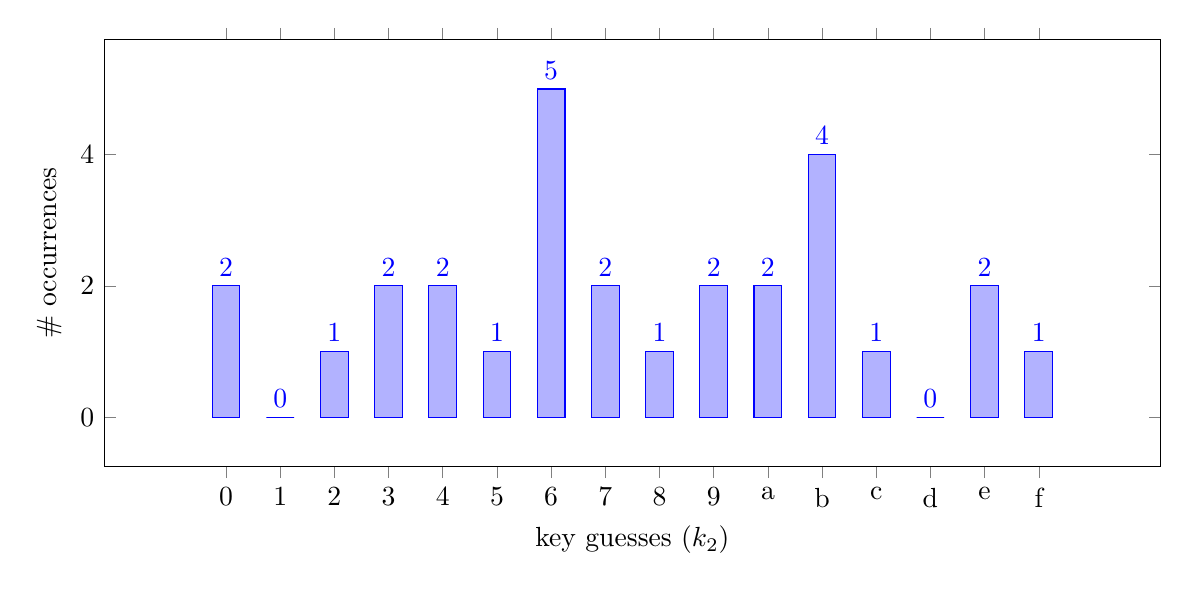
\begin{tikzpicture}

\begin{axis}
[
ybar,
symbolic x coords={0,1,2,3,4,5,6,7,8,9,a,b,c,d,e,f},
enlargelimits=0.15,
xtick=data,
nodes near coords,
nodes near coords align={vertical},
xlabel={key guesses ($k_2$)},
ylabel={\# occurrences}
]
\addplot+[ybar, mark=no] coordinates {
(0,2) (1,0) (2,1) (3,2) (4,2) (5,1) (6,5) (7,2) (8,1) (9,2) (a,2) (b,4) (c,1) (d,0) (e,2) (f,1)
};
\end{axis}

\end{tikzpicture}

\end{center}

From the matrix and SNR graph, it is evident that the signal for $k_2$ = 6 is highest, which is correct given our selection of keys.

\end{large}

\section{Hamsi vs CryptWizard001}
\begin{large}
The Hamsi S-box is:
\begin{center}

\begin{tabular}{|c|c|c|c|c|c|c|c|c|c|c|c|c|c|c|c|c|}
\hline
$x$ & 0 & 1 & 2 & 3 & 4 & 5 & 6 & 7 & 8 & 9 & a & b & c & d & e & f\\\hline
$S(x)$ & 8 & 6 & 7 & 9 & 3 & c & a & f & d & 1 & e & 4 & 0 & b & 5 & 2\\\hline
\end{tabular}

\end{center}

\vspace{1cm}
The DDT for Hamsi S-box is:

\begin{center}

\begin{tabular}{c||*{16}{p{0.5cm}}}
in\textbackslash out & 0 & 1 & 2 & 3 & 4 & 5 & 6 & 7 & 8 & 9 & a & b & c & d & e & f\\\hline
0 & 16 & - & - & - & - & - & - & - & - & - & - & - & - & - & - & - \\
1 & - & - & - & - & - & 2 & - & 2 & - & - & 2 & 2 & 2 & - & 4 & 2 \\
2 & - & - & - & 4 & - & 4 & - & - & - & 4 & - & - & - & - & - & 4 \\
3 & - & 4 & 2 & - & - & - & 2 & - & - & 2 & - & - & 2 & - & 2 & 2 \\
4 & - & - & - & - & - & - & 4 & - & - & - & 4 & 4 & - & 4 & - & - \\
5 & - & 4 & - & 2 & 2 & 2 & 2 & - & 2 & - & - & - & 2 & - & - & - \\
6 & - & - & 2 & 2 & 2 & 2 & - & - & 2 & 2 & - & - & - & - & 2 & 2 \\
7 & - & - & - & - & 4 & 2 & - & 2 & - & - & 2 & 2 & 2 & - & - & 2 \\
8 & - & - & - & 2 & - & 2 & - & 4 & - & 2 & - & - & - & 4 & - & 2 \\
9 & - & - & - & 2 & - & - & - & 2 & 4 & 2 & 2 & 2 & 2 & - & - & - \\
a & - & - & 2 & - & 2 & - & 4 & - & 2 & - & 4 & - & - & - & 2 & - \\
b & - & 4 & - & - & 2 & - & 2 & - & 2 & 2 & - & - & 2 & - & - & 2 \\
c & - & - & 2 & - & 2 & - & - & - & 2 & - & - & 4 & - & 4 & 2 & - \\
d & - & 4 & 2 & 2 & - & 2 & 2 & - & - & - & - & - & 2 & - & 2 & - \\
e & - & - & 2 & - & 2 & - & - & 4 & 2 & - & - & - & - & 4 & 2 & - \\
f & - & - & 4 & 2 & - & - & - & 2 & - & 2 & 2 & 2 & 2 & - & - & - \\

\end{tabular}

\end{center}

There are 72 places with entry:"2" and 24 with entry:"4".


CryptWizard001's S-box is:

\begin{center}

\begin{tabular}{|c|c|c|c|c|c|c|c|c|c|c|c|c|c|c|c|c|}
\hline
$x$ & 0 & 1 & 2 & 3 & 4 & 5 & 6 & 7 & 8 & 9 & a & b & c & d & e & f\\\hline
$S(x)$ & c & 6 & 7 & 9 & 4 & 8 & a & f & 5 & 1 & e & 3 & 0 & b & d & 2\\\hline
\end{tabular}

\end{center}

The DDT for CryptWizard001's S-box is:

\begin{center}

\begin{tabular}{c||*{16}{p{0.5cm}}}
in\textbackslash out & 0 & 1 & 2 & 3 & 4 & 5 & 6 & 7 & 8 & 9 & a & b & c & d & e & f\\\hline
0 & 16 & - & - & - & - & - & - & - & - & - & - & - & - & - & - & - \\
   1 & - & - & - & - & 2 & 2 & - & - & - & - & 2 & 2 & 2 & 2 & 2 & 2 \\
   2 & - & - & 2 & - & - & - & - & 2 & - & 2 & - & 4 & - & 2 & 2 & 2 \\
   3 & - & 2 & 4 & - & - & 2 & 4 & - & - & - & - & 2 & - & - & - & 2 \\
   4 & - & 2 & - & 2 & - & 2 & 2 & - & 2 & - & 2 & - & - & 2 & 2 & - \\
   5 & - & 2 & 2 & 2 & 2 & - & - & - & 2 & - & - & - & 2 & - & 4 & - \\
   6 & - & 2 & - & 4 & - & - & 2 & - & 4 & 2 & - & - & - & - & 2 & - \\
   7 & - & - & - & 4 & - & 2 & - & 2 & - & - & - & - & 4 & 2 & - & 2 \\
   8 & - & - & - & 2 & 2 & - & - & 4 & - & 4 & 2 & - & - & 2 & - & - \\
   9 & - & - & 2 & 2 & 2 & - & - & 2 & 4 & - & - & - & - & 2 & - & 2 \\
   a & - & - & 4 & - & 2 & 2 & - & - & 2 & 2 & 4 & - & - & - & - & - \\
   b & - & 2 & - & - & - & 2 & 4 & - & 2 & - & - & - & 2 & - & - & 4 \\
   c & - & 2 & - & - & 2 & - & - & - & - & 2 & 2 & 2 & 4 & 2 & - & - \\
   d & - & 2 & - & - & 2 & 4 & 2 & 2 & - & 2 & - & - & - & 2 & - & - \\
   e & - & 2 & 2 & - & 2 & - & - & 2 & - & - & 2 & 2 & - & - & 2 & 2 \\
   f & - & - & - & - & - & - & 2 & 2 & - & 2 & 2 & 4 & 2 & - & 2 & - \\
\end{tabular}

\end{center}

There are 84 places with entry:"2" and 18 with entry:"4".\\

A fixed point in an S-Box is a property where S[x] = x. For CryptWizard001's S-Box, there is one fixed point, where S[4] = 4. This can be used to launch Fixed Point Attack on ciphers (Bard G.V. (2009) The Fixed-Point Attack. In: Algebraic Cryptanalysis. Springer, Boston, MA, pp 17-28). Algorithms that generate highly secure and non-linear S-Boxes work to avoid creating fixed points.

Since CryptWizard001's S-Box creats a fixed point, it is more vulnerable to attacks. Hence, CryptWizard001 is a liar.

\end{large}
\vspace{0.5cm}

\section{Conforming Message Pairs}
\begin{large}

The 16-bits keys used for Sypher004 are = ('c253', '0466', 'affe', '645e', '0509', 'fff2').\\
Python code (Python 3): conform\textunderscore msg.py

\lstinputlisting[language = Python, showstringspaces=false]{./python_code/conform_msg.py}

Actual output (file generated by code contains conforming message pairs and cipher pairs): output\textunderscore cnfrm.txt

Number of conforming message pairs = 356\\
$\therefore$ Probability of differential $(8,0,0,0) \xrightarrow{S} ? \xrightarrow{S} (8,0,0,0)$ = $\dfrac{356}{2^{16}}$ = $0.00543$.

The conditions for filtering here are to remove message-pairs which activate S-Boxes for nibbles 2,3 and 4, as well as those which give differences that do not match that of differential for S-Box 1.

\end{large}


\end{document}